\documentclass{article}
\usepackage{amsmath}
\usepackage{mathtools}
\usepackage{gensymb}
\usepackage[a4paper,inner=1.5cm,outer=1.5cm,top=2cm,bottom=0.5cm]{geometry} 
\usepackage{xcolor}                    
\usepackage{tikz}                           
\usepackage{multicol}
\usepackage{hyperref}
\usepackage{pgfplots}
\usetikzlibrary{calc}
\usetikzlibrary{intersections}
\usetikzlibrary{intersections,calc,angles,quotes}
\usetikzlibrary{shapes,arrows,positioning,decorations.pathreplacing,calc}
\usetikzlibrary{calc,angles,positioning,intersections,quotes,decorations.markings}
\usepackage{tkz-euclide}
\usetikzlibrary{backgrounds}
\usetikzlibrary{calc,through}
\usetikzlibrary{angles}
\usetikzlibrary{fadings}
\usetikzlibrary{shapes.geometric}
\usetikzlibrary{shapes.symbols}
\usepackage{draftwatermark}
\usepackage{mathptmx}

\SetWatermarkText{\textcolor{black!20}{Mathema Shukur}}
\SetWatermarkFontSize{2 cm}
\usepackage[utf8]{inputenc}
\usepackage{fontspec}

\setmainfont{[Kalpurush.ttf]}
\newfontface{\en}{[Arial.ttf]} %%this is optional, if you want to use a secondary font. Any english font is supported
\newlength\Radius
\setlength\Radius{4cm}
\begin{document} 
	\Large
	\textcolor{red}{Welcome To} 
	\\
	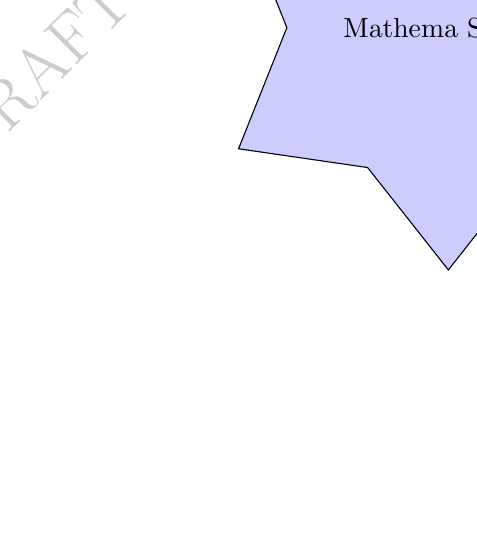
\begin{tikzpicture}
		\tikz \node [fill=blue!20,star,star points=6,draw] {Mathema Shukur };
	\end{tikzpicture}
	\\
	যাদের জন্যে প্রযোজ্যঃ  	\textcolor{magenta}{একাদশ ও দ্বাদশ শ্রেণীর শিক্ষার্থী} \\
	বিষয়ঃ \textcolor{magenta}{উচ্চতর গণিত ১ম পত্র} \\
	অধ্যায়ঃ \textcolor{magenta}{৪-বৃত্ত}\\ 
	\\
	(1a) $(x_1,y_1)$ বিন্দু হতে   $x^2+y^2=a^2$  বৃত্তে অঙ্কিত স্পর্শকের দৈর্ঘ্য \\
	$\sqrt{x_1^2+y_1^2-a^2}$\\
	\\ 
	(1b) $(x_1,y_1)$ বিন্দু হতে  $x^2+y^2+2gx+2fy+c=0$  বৃত্তে অঙ্কিত স্পর্শকের দৈর্ঘ্য \\   $\sqrt{x_1^2+y_1^2+2gx_1+2fy_1+c}$\\
	\\
	\textcolor{blue}{কুমিল্লা বোর্ড-২০২৩}\\ 	
		$(1,-1)$ বিন্দু হতে  $x^2+y^2-12x+30=0$ বৃত্তে অঙ্কিত স্পর্শকের দৈর্ঘ্য নির্ণয় কর।  \\
			\\ 
			\begin{align*}
				x^2+y^2-12x+30&=0\\
				\\
				\boxed{\textcolor{blue}{x^2+y^2+2gx+2fy+c=0}}&\\
				\\
					x^2+y^2+2(-6)x+2(0)y+30&=0\\
					\\
					g=-6,\,\,f=0,\,\,c=30&
			\end{align*}
		\\
		\\
	 $x^2+y^2-12x+30=0$ বৃত্তে অঙ্কিত স্পর্শকের দৈর্ঘ্য \\ 
		\begin{align*}
	&	\sqrt{x_1^2+y_1^2+2gx_1+2fy_1+c}\\
		\\
	&	\boxed{\textcolor{blue}{x_1=1,\,\,y_1=-1,\,\,g=-6,\,\,f=0,\,\,c=30}}
		\\
			&=	\sqrt{(1)^2+(-1)^2+2(-6)(1)+2(0)(-1)+30}\\
			\\
				&=	\sqrt{1+1-12+0+30}\\
				\\
			&=	\sqrt{20}\\	
			\\
			&=2	\sqrt{5}\\		
		\end{align*}
	\\
	 $x^2+y^2-12x+30=0$ বৃত্তে অঙ্কিত স্পর্শকের দৈর্ঘ্য $AB=AC=2\sqrt{5}$\\ 
	 \\
	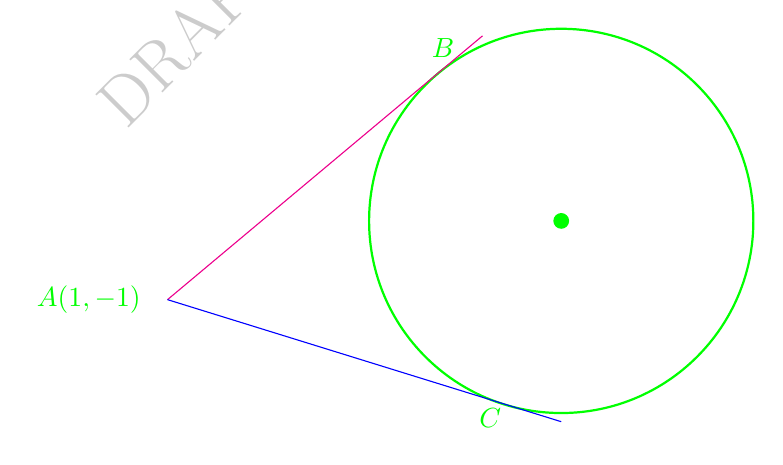
\begin{tikzpicture}[transform shape,scale=1]
		\draw[thick,green] (6,0) circle (2.44);
		\fill[green] (6,0) circle (1 mm);
		\draw[magenta](1,-1)--(5,2.35);
		\draw[blue](1,-1)--(6,-2.55);
		\node at (0,-1) {$\textcolor{green}{A(1,-1)}$};	
		\node at (4.5,2.2) {$\textcolor{green}{B}$};
		\node at (5.1,-2.5) {$\textcolor{green}{C}$};					
	\end{tikzpicture}\\
	\\
		\textcolor{blue}{কুমিল্লা বোর্ড-২০২২}  \\ 	
		$(2,2)$ বিন্দু হতে  $x^2+y^2+4x-2y+4=0$ বৃত্তে অঙ্কিত স্পর্শকের দৈর্ঘ্য নির্ণয় কর।  \\
			\\ 
			\\ 
			\begin{align*}
				x^2+y^2+4x-2y+4&=0\\
				\\
				\boxed{\textcolor{blue}{x^2+y^2+2gx+2fy+c=0}}&\\
				\\
				x^2+y^2+2(2)x+2(-1)y+4&=0\\
				\\
				g=2,\,\,f=-1,\,\,c=4&
			\end{align*}
			\\
			$x^2+y^2+4x-2y+4=0$ বৃত্তে অঙ্কিত স্পর্শকের দৈর্ঘ্য\\
			\\
			\begin{align*}
				&	\sqrt{x_1^2+y_1^2+2gx_1+2fy_1+c}\\
				\\
				&	\boxed{\textcolor{blue}{x_1=2,\,\,y_1=2,\,\,g=2,\,\,f=-1,\,\,c=4}}
				\\
				&=	\sqrt{(2)^2+(2)^2+2(2)(2)+2(-1)(2)+4}\\
				\\
				&=	\sqrt{4+4+8-4+4}\\
				\\
				&=	\sqrt{16}\\	
				\\
				&=4	\\		
			\end{align*}
		$x^2+y^2+4x-2y+4=0$ বৃত্তে অঙ্কিত স্পর্শকের দৈর্ঘ্য $AB=AC=4$\\
		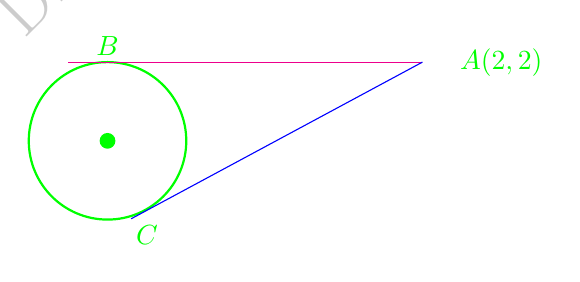
\begin{tikzpicture}[transform shape,scale=1]
			\draw[thick,green] (-2,1) circle (1);
			\fill[green] (-2,1) circle (1 mm);
			\draw[magenta](2,2)--(-2.5,2);
			\draw[blue](2,2)--(-1.7,0.01);
				\node at (3,2) {$\textcolor{green}{A(2,2)}$};	
			\node at (-2,2.2) {$\textcolor{green}{B}$};	
			\node at (-1.5,-0.2) {$\textcolor{green}{C}$};			
		\end{tikzpicture}\\
		\\
		\textcolor{blue}{বরিশাল বোর্ড-২০২২}  \\ 	
		$(3,1)$ বিন্দু হতে  $2x^2+2y^2=18$ বৃত্তে অঙ্কিত স্পর্শকের দৈর্ঘ্য নির্ণয় কর।  \\
		\\
		\textcolor{blue}{রাজশাহী বোর্ড-২০২২}\\ 	
		$(1,1)$ বিন্দু হতে  $2x^2+2y^2-x+3y+1=0$ বৃত্তে অঙ্কিত স্পর্শকের দৈর্ঘ্য নির্ণয় কর।  \\
		\\
		\textcolor{blue}{সিলেট বোর্ড-২০২২}\\ 	
		$(-1,-3)$ বিন্দু হতে  $x^2+y^2-2x-y-7=0$ বৃত্তে অঙ্কিত স্পর্শকের দৈর্ঘ্য নির্ণয় কর।  \\
		\\
			\textcolor{blue}{কুমিল্লা বোর্ড-২০২৩}\\  
			$(0,0)$ মূল বিন্দু থেকে $x^2+y^2+2x+3y+1=0$ বৃত্তে অঙ্কিত স্পর্শকের সমীকরণ ও দৈর্ঘ্য নির্ণয় কর। \\ 
		\\ 
			\textcolor{blue}{সকল বোর্ড-২০১৮}\\
		$(-5,4)$ বিন্দু থেকে $x^2+y^2-2x-4y+1=0$ বৃত্তে অঙ্কিত স্পর্শকের সমীকরণ নির্ণয় কর। \\ 
	\\
	\begin{align*}
	x^2+y^2-2x-4y+1&=0\\
		\boxed{\textcolor{blue}{x^2+y^2+2gx+2fy+c=0}}&\\
		x^2+y^2+2(-1)x+2(-2)y+(1)&=0
	\end{align*}
	\\
	কেন্দ্র 	$(-g,-f)=(1,2)$ ও ব্যাসার্ধ= $\sqrt{(-1)^2+(-2)^2-1}=\sqrt{1+4-1}=2$\\
	\\ 
	$(-5,4)$ বিন্দুগামী সরলরেখার সমীকরণ \\ 
	\begin{align*}
		(y-y_1)&=m(x-x_1)\\
	&	\boxed{\textcolor{blue}{x_1=-5,\,\,y_1=4}}\\
		y-4&=m(x+5)\,\,\,[EQ01]\\
		\\
		y-4&=mx+5m\\
		\\
		mx-y+5m+4&=0
	\end{align*}
	\textcolor{blue}{$P(x_1,y_1)$ বিন্দু হতে  $ax+by+c=0$ সরলরেখার উপর অঙ্কিত লম্বের দৈর্ঘ্য বা লম্ব দূরত্ব \\
		\\
		$d=\frac{|ax_1+by_1+c|}{\sqrt{a^2+b^2}}$}\\
	\\
	কেন্দ্র \textcolor{green}{$(1,2)$} হতে \textcolor{magenta}{$mx-y+5m+4=0$}  রেখার লম্ব দূরত্ব= $	\frac{|m(1)-2+5m+4|}{\sqrt{(m)^2+(-1)^2}}$\\
	\\ 
	\textcolor{blue}{কেন্দ্র হতে স্পর্শকের লম্ব দূরত্ব= ব্যাসার্ধ}\\ 
	\begin{multicols}{2}
\begin{align*}
	\frac{|m(1)-2+5m+4|}{\sqrt{(m)^2+(-1)^2}}&=2\\
	\frac{|m-2+5m+4|}{\sqrt{m^2+1}}&=2\\
	\frac{|6m+2|}{\sqrt{m^2+1}}&=2\\
	\\
	\frac{6m+2}{\sqrt{m^2+1}}&=\pm 2\\
	\\
	\frac{3m+1}{\sqrt{m^2+1}}&=\pm 1\\
\end{align*}
\\
\begin{align*}
	(3m+1)^2&=m^2+1\\
	\\
	9m^2+6m+1&=m^2+1\\
	\\
	8m^2+6m&=0\\
	\\
	2m(4m+3)&=0\\
	\\
	m=0,\,\,\,m&=-\frac{3}{4}
\end{align*}
	\end{multicols}
\begin{multicols}{2}
	\begin{align*}
	y-4&=m(x+5)\,\,\,[EQ01]\\
	&	\boxed{\textcolor{blue}{m=0}}\\
	y-4&=(0)(x+5)\\
	\\
	y-4&=0
\end{align*}
\\
\begin{align*}
	y-4&=m(x+5)\,\,\,[EQ01]\\
	&	\boxed{\textcolor{blue}{m=-\frac{3}{4}}}\\
	y-4&=-\frac{3}{4}(x+5)\\
	\\
	4y-16&=-3x-15\\
	\\
	3x+4y-1&=0
\end{align*}
\end{multicols}
স্পর্শক $AB$ এর সমীকরণ  $y-4=0$\\
\\
স্পর্শক $AC$ এর সমীকরণ $3x+4y-1=0$\\ 
\\
	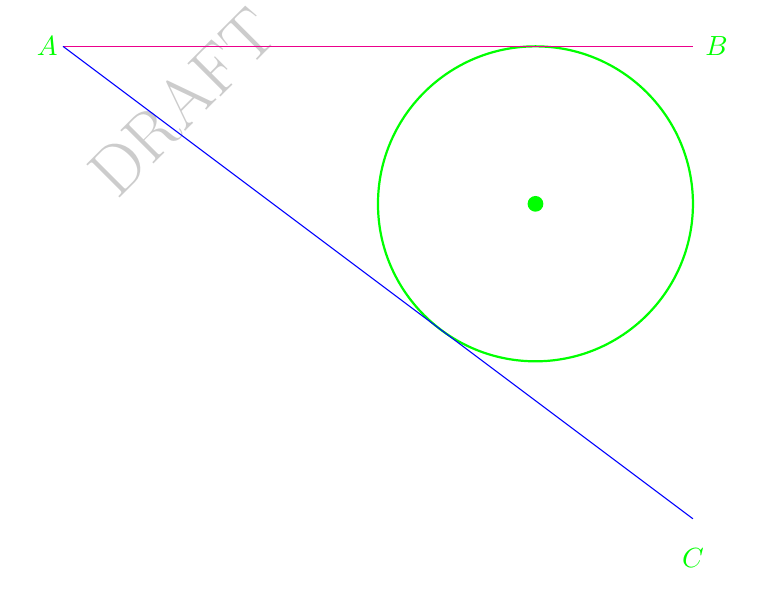
\begin{tikzpicture}[transform shape,scale=1]
		\draw[thick,green] (1,2) circle (2);
		\fill[green] (1,2) circle (1 mm);
		\draw[magenta](-5,4)--(3,4);
		\draw[blue](-5,4)--(3,-2);
		\node at (-5.2,4) {$\textcolor{green}{A}$};		
		\node at (3.3,4) {$\textcolor{green}{B}$};		
		\node at (3,-2.5) {$\textcolor{green}{C}$};			
	\end{tikzpicture}\\
\end{document}